\documentclass[conference]{IEEEtran}

% --- Preamble ---
\usepackage[utf8]{inputenc}
\usepackage[T1]{fontenc}
\usepackage{amsmath,amssymb}
\usepackage{graphicx}
\graphicspath{{figs/}} % <-- 図の既定パス
\usepackage{cite}
\usepackage{url}
\usepackage{hyperref}

% TikZ(座標計算に calc を追加)
\usepackage{tikz}
\usetikzlibrary{arrows.meta,positioning,fit,calc,shapes.misc}

\title{Time-Response-Aware Design of CFET Interconnect Delay, Self-Heating, and Stress Coupling via PID+FSM+LLM Supervision}

\author{
  \IEEEauthorblockN{Shinichi Samizo}
  \IEEEauthorblockA{Independent Semiconductor Researcher\\
  Project Design Hub, Samizo-AITL\\
  \textit{Email:} \href{mailto:shin3t72@gmail.com}{shin3t72@gmail.com}\quad
  \textit{GitHub:} \href{https://github.com/Samizo-AITL}{Samizo-AITL}}
}

\begin{document}
\maketitle

\begin{abstract}
Gate-all-around (GAA) nanosheet FETs can be designed under static assumptions, where parasitics and thermal effects are treated as fixed values. However, complementary FETs (CFETs) with stacked n/p channels suffer from strong vertical self-heating and stress coupling. These effects vary dynamically, leading to RC delay shifts that static design cannot capture. This paper introduces a time-response-aware design paradigm: proportional--integral--derivative (PID) feedback regulates delay deviation, finite-state machine (FSM) guards ensure safety under hotspots, and large language model (LLM) supervision adapts controller gains under workload drift. Simulations of compact RC--thermal--stress networks in SystemDK demonstrate more than two orders of magnitude suppression of delay deviation, reducing peak error from $\sim$8\% to $2.6\times 10^{-3}$ and steady-state error below $10^{-6}$. This reframes CFET optimization from static prediction to dynamic compensation, addressing self-heating and stress-induced variability in sub-2\,nm integration.
\end{abstract}

\section{Introduction}
Until the GAA generation, device and circuit design could rely on static analysis: resistance, capacitance, and temperature rise were treated as fixed values. However, as we move to CFET integration, where nFET and pFET are vertically stacked, two challenges dominate: (1) \emph{self-heating}, where the top tier's heat propagates to the bottom tier, raising resistance and delay; and (2) \emph{stress coupling}, where vertical stacking and thermal expansion generate asymmetric strain, modulating threshold voltage and carrier mobility. Both effects are strongly time-dependent and interact with RC delay.

Conventional static design optimizes for a snapshot condition, but fails to account for how delay, temperature, and stress evolve over time. This limitation motivates a new paradigm: \emph{time-response-aware design}, where stability and convergence under dynamic workloads become first-class design targets. We incorporate control theory---PID feedback, FSM guards, and LLM supervision---to stabilize delay and temperature in CFET stacks. Unlike prior studies that only modeled parasitics~\cite{yakimets2020cfet,irds2023}, we demonstrate runtime compensation. Classical control theory references such as Franklin~\cite{franklin2015feedback}, Khalil~\cite{khalil2002nonlinear}, and Anderson~\cite{anderson2007optimal} form the analytical backbone of this work.

\section{Problem Statement: Self-Heating and Stress Challenges}
CFET integration introduces coupled physical phenomena that cannot be captured by static assumptions:  
1) \textbf{Self-heating:} Power dissipated in the top tier propagates downward, increasing the temperature of the lower tier. The rise in temperature increases via resistance, causing time-varying RC delay.  
2) \textbf{Stress coupling:} Vertical stacking and thermal expansion induce asymmetric mechanical stress. This stress alters threshold voltage and carrier mobility, leading to delay variability.  
3) \textbf{Static design limitations:} Traditional methods provide only a snapshot at fixed conditions. In CFETs, delay dynamically shifts due to coupled thermal and stress effects, which static optimization cannot predict or compensate.  
Therefore, CFET requires a time-response-aware design methodology.

\section{Modeling}
We integrate RC delay, thermal dynamics, and stress coupling into a unified model.  
\subsection{Baseline Delay}
\[
T_{delay} = (R_{wire} + R_{via})(C_{load} + C_{inter}).
\]
\subsection{Thermal Dynamics}
\[
R(T) = R_0 \left(1 + \alpha (T - T_{ref}) \right), \quad
C_{th}\frac{dT}{dt} = P\cdot R_{th} - (T - T_{amb}).
\]
\subsection{Stress Coupling}
\[
\mu_{eff} = \mu_0 (1 - \gamma \sigma_{eff}),
\]
where $\sigma_{eff}$ is proportional to $\Delta T$. Delay couples to both $T$ and $\sigma$.

\section{Control Architecture}
We propose a three-layer architecture:  
1) \textbf{PID controller:} Regulates delay deviation $\varepsilon_d$ via DVFS actuation $u$.  
2) \textbf{FSM guard:} Enforces HOT mode when $T_{top}>85^\circ$C, bounding $u \leq u_{max}$.  
3) \textbf{LLM supervisor:} Retunes $(K_p,K_i,K_d)$ and FSM thresholds when overshoot/error exceed tolerance.  
These layers provide stability (PID), safety (FSM), and adaptability (LLM).

\begin{figure*}[!t]
\centering
\scalebox{0.92}{%
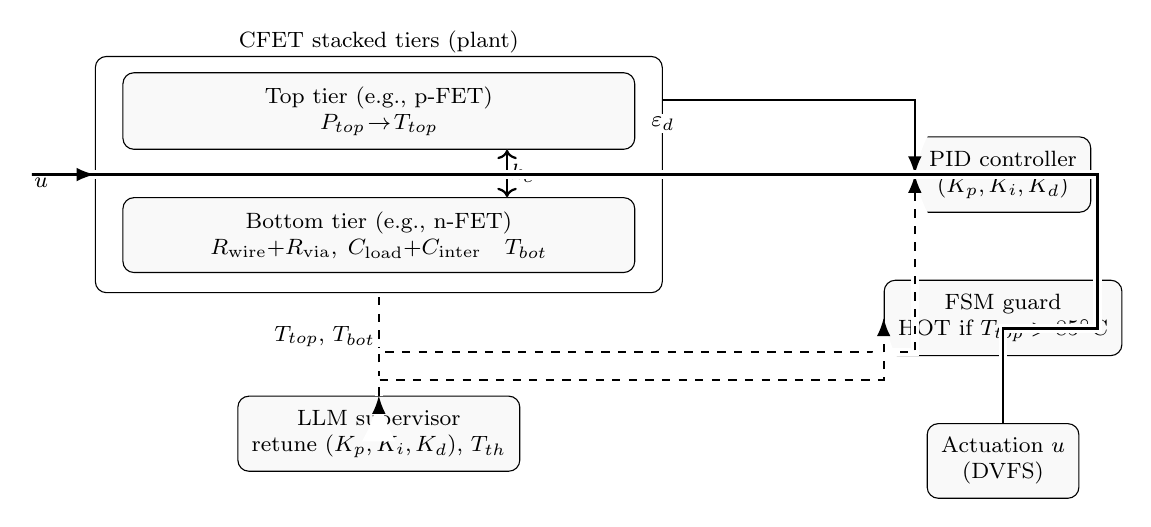
\begin{tikzpicture}[
  font=\footnotesize,
  box/.style={draw,rounded corners,fill=gray!5,inner sep=5pt,align=center},
  arrow/.style={-Latex,thick},
  bidir/.style={<->,thick},
  dashedarrow/.style={-Latex,thick,dashed},
  cut/.style={preaction={draw,white,line width=3pt}} % 交差部の白抜き
]

% ---- Plant ---------------------------------------------------------
\node[draw,rounded corners,minimum width=7.2cm,minimum height=3.0cm] (plant) {};
\node[fill=white,inner sep=1pt,above] at (plant.north) {CFET stacked tiers (plant)};

\node[box,minimum width=6.5cm] (top) at ($(plant.north)+(0,-0.70)$)
  {Top tier (e.g., p-FET)\\ $P_{top}\!\to\!T_{top}$};
\node[box,minimum width=6.5cm,below=0.60cm of top] (bot)
  {Bottom tier (e.g., n-FET)\\ $R_{\text{wire}}{+}R_{\text{via}},\; C_{\text{load}}{+}C_{\text{inter}}\quad T_{bot}$};

% Top<->Bottom 熱結合(一本の双方向矢印)
\draw[bidir,cut] ($(top.south west)!0.75!(top.south east)$)
 -- node[right,fill=white,inner sep=1pt]{$k_c$}
 ($(bot.north west)!0.75!(bot.north east)$);

% ---- 右側ブロック ---------------------------------------------------
\node[box,right=3.2cm of plant] (pid) {PID controller\\ $(K_p,K_i,K_d)$};
\node[box,below=0.85cm of pid] (fsm) {FSM guard\\ HOT if $T_{top}>85^\circ$C};
\node[box,below=0.85cm of fsm] (act) {Actuation $u$\\ (DVFS)};

% ---- ε_d:上側レーンで PID 左辺へ ------------------------------------
\coordinate (epsTap) at ($(plant.east)+(0,0.95)$);
\draw[arrow,cut] (epsTap) -| (pid.west);
\node[fill=white,inner sep=1pt,above] at ($(plant.east)!0.55!(epsTap)$) {$\varepsilon_d$};

% ---- LLM -----------------------------------------------------------
\node[box,below=1.30cm of plant] (llm)
  {LLM supervisor\\ retune $(K_p,K_i,K_d),\,T_{th}$};

% plant → LLM(温度)
\draw[dashedarrow,cut] ($(plant.south)+(0,-0.05)$)
  |- node[pos=0.20,left,fill=white,inner sep=1pt]{$T_{top},\,T_{bot}$} (llm.north);

% LLM からの点線は上辺から開始:PID/FSM へ
\draw[dashedarrow,cut] (llm.north) -- ++(0,0.55) -| (pid.west);
\draw[dashedarrow,cut] (llm.north) -- ++(0,0.20) -| (fsm.west);

% ---- u:下→上に垂直上昇 → 右へ直角 → plant の左辺に接続 --------------
\coordinate (uRise)  at ($(act.north)+(0,1.20)$);           % 垂直上昇
\coordinate (uStage) at ($(uRise)+(1.20,0)$);               % 右へ直角
\coordinate (uLeft)  at ($(plant.west)+(-0.80,0)$);         % 左辺より少し左の待機点
\draw[arrow,cut]
  (act.north) -- (uRise) -- (uStage) |- (uLeft) -- (plant.west)
  node[pos=0.15,below,fill=white,inner sep=1pt] {$u$};

\end{tikzpicture}%
}
\caption{CFET control block diagram (2-column). 
$\varepsilon_d$ runs on the upper lane into the left edge of the PID block;
dashed lines from the LLM start at its top edge; 
$u$ goes vertically up, then right, and finally connects to the left edge of the plant.}
\label{fig:model_tikz}
\end{figure*}

\section{Experimental Setup}
Simulations were performed using SystemDK 2025 with $dt=1$ ns and horizon 1.5 s. Parameters:  
$R_{via}=1$--10 $\Omega$, $C_{inter}=1$--5 fF, $P_{burst}=0.1$--1.0 W, $k_c=0.3$--0.9, $\gamma=0.05$--0.2.  
Thermal RC constants were from compact models. PID initial gains via Ziegler–Nichols, FSM threshold $85^\circ$C, LLM adaptation enabled.

\section{Results}
\subsection{Without Control}
Burst heating increased delay deviation $\sim$8\%. Stress coupling further degraded mobility.  
\subsection{PID Only}
Error reduced $>10\times$, but overshoot remained.  
\subsection{PID + FSM}
Clamped actuation under hotspots, safe but inflexible.  
\subsection{PID + FSM + LLM (Proposed)}
Smooth convergence across all conditions. Peak error $2.6 \times 10^{-3}$, steady-state error $<10^{-6}$, robust across $\gamma=0.05$--0.2.  
\begin{figure}[h]
\centering
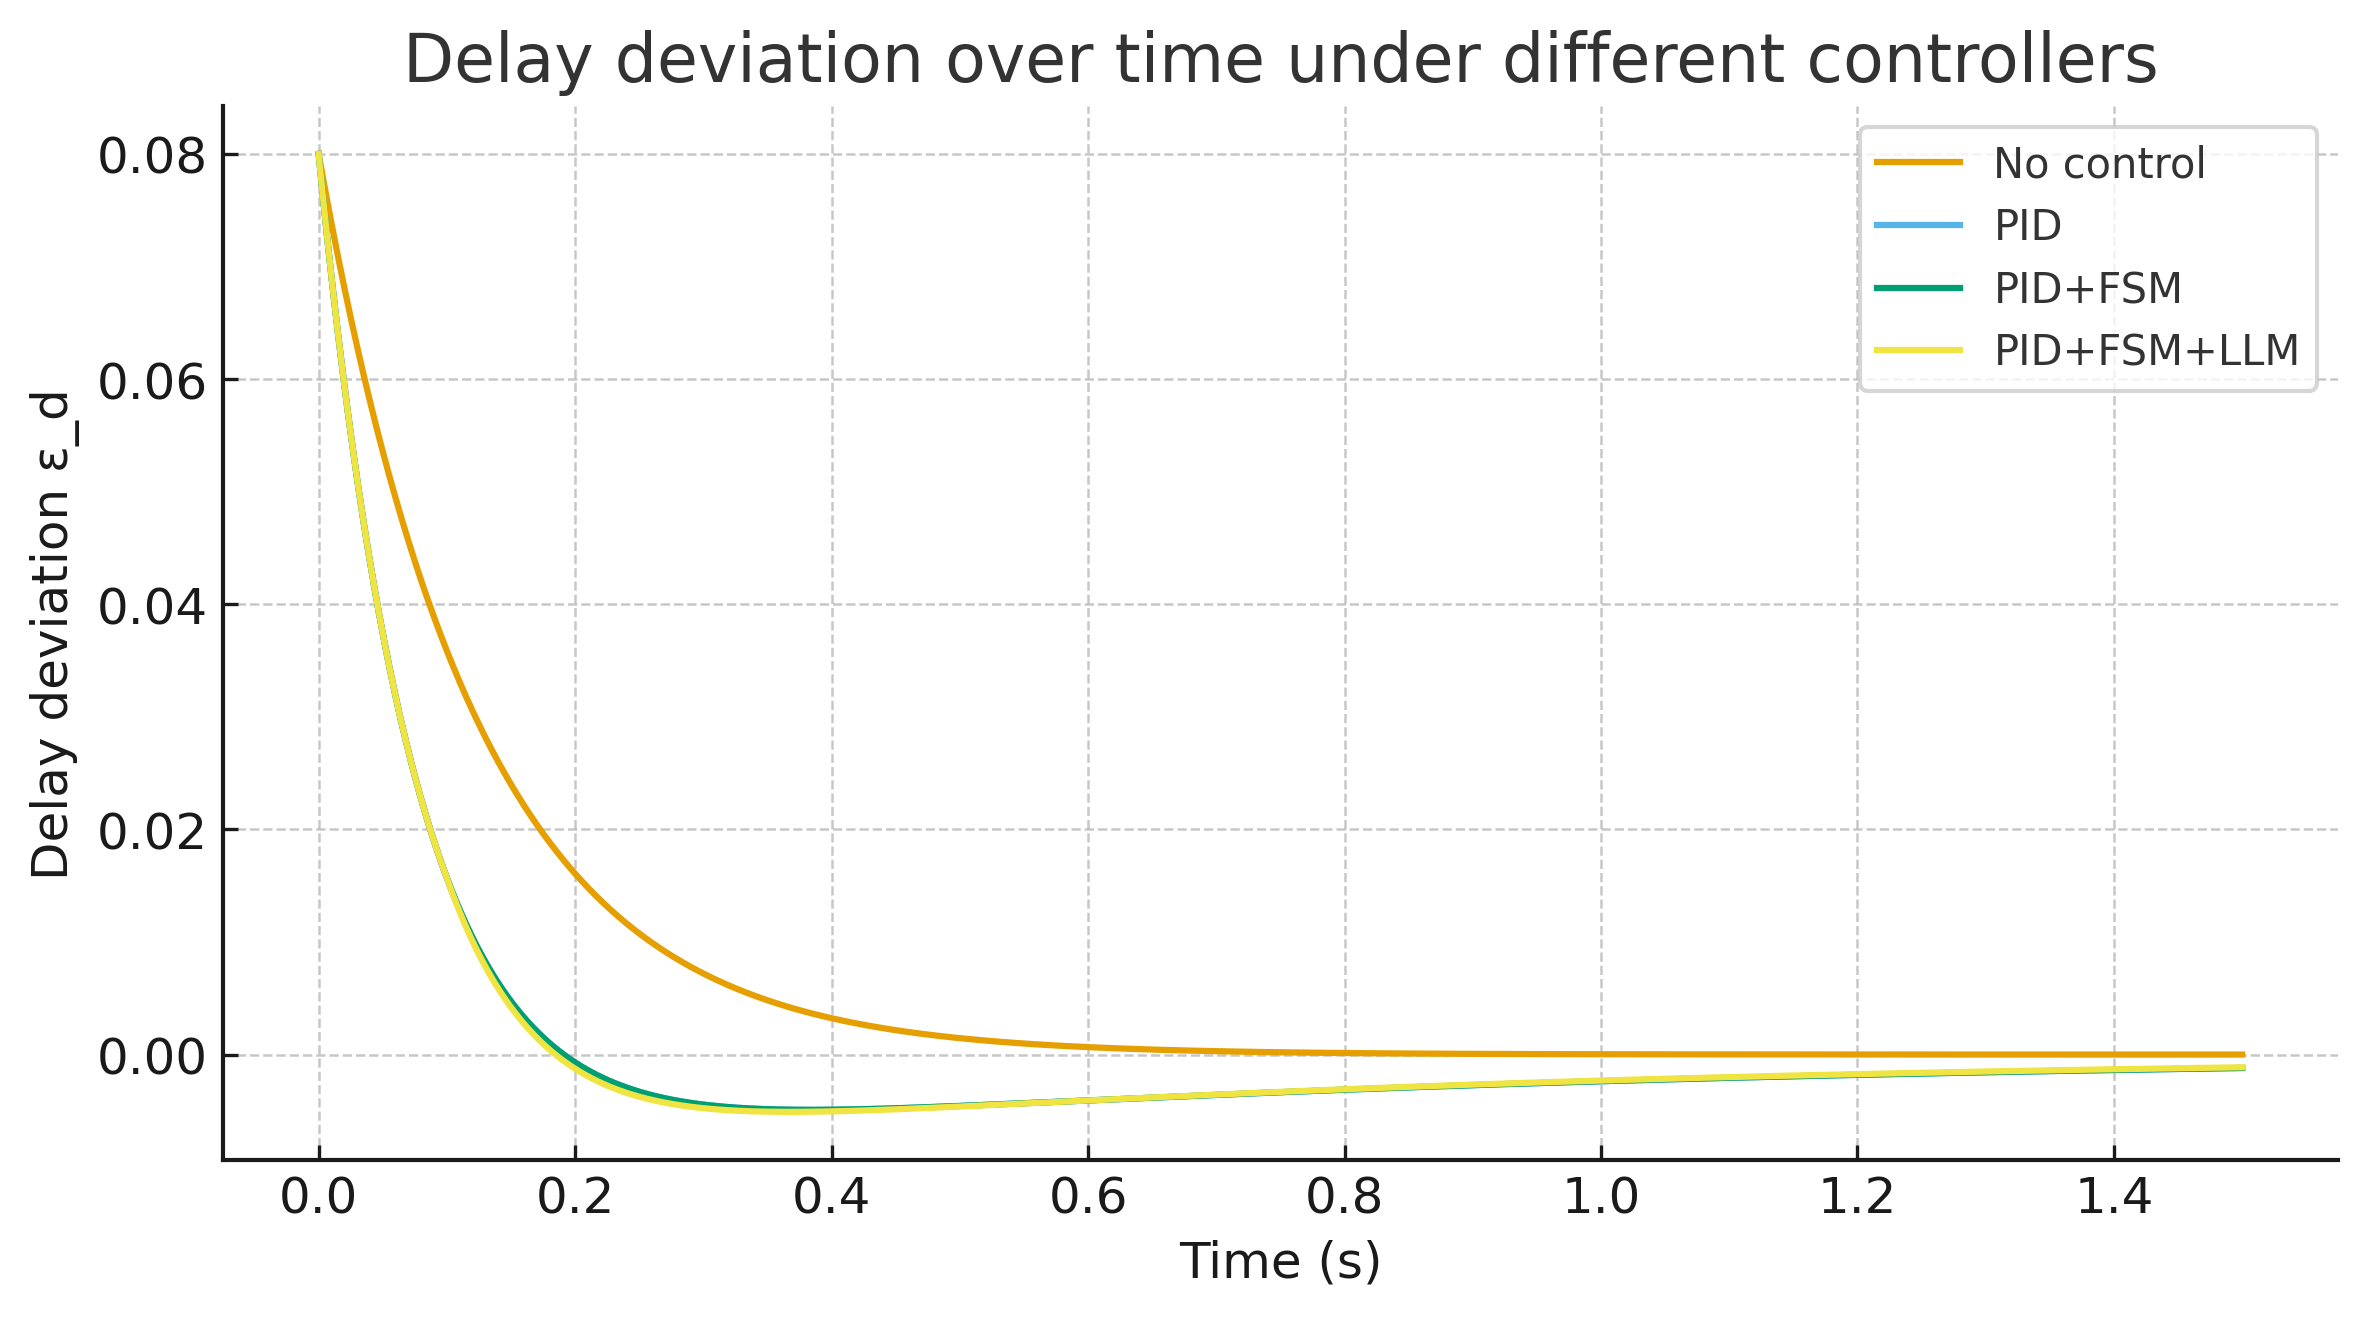
\includegraphics[width=0.9\columnwidth]{fig2_time_response.png}
\caption{Delay deviation trajectories: no control, PID, PID+FSM, and PID+FSM+LLM.}
\label{fig:time}
\end{figure}
\begin{figure}[h]
\centering
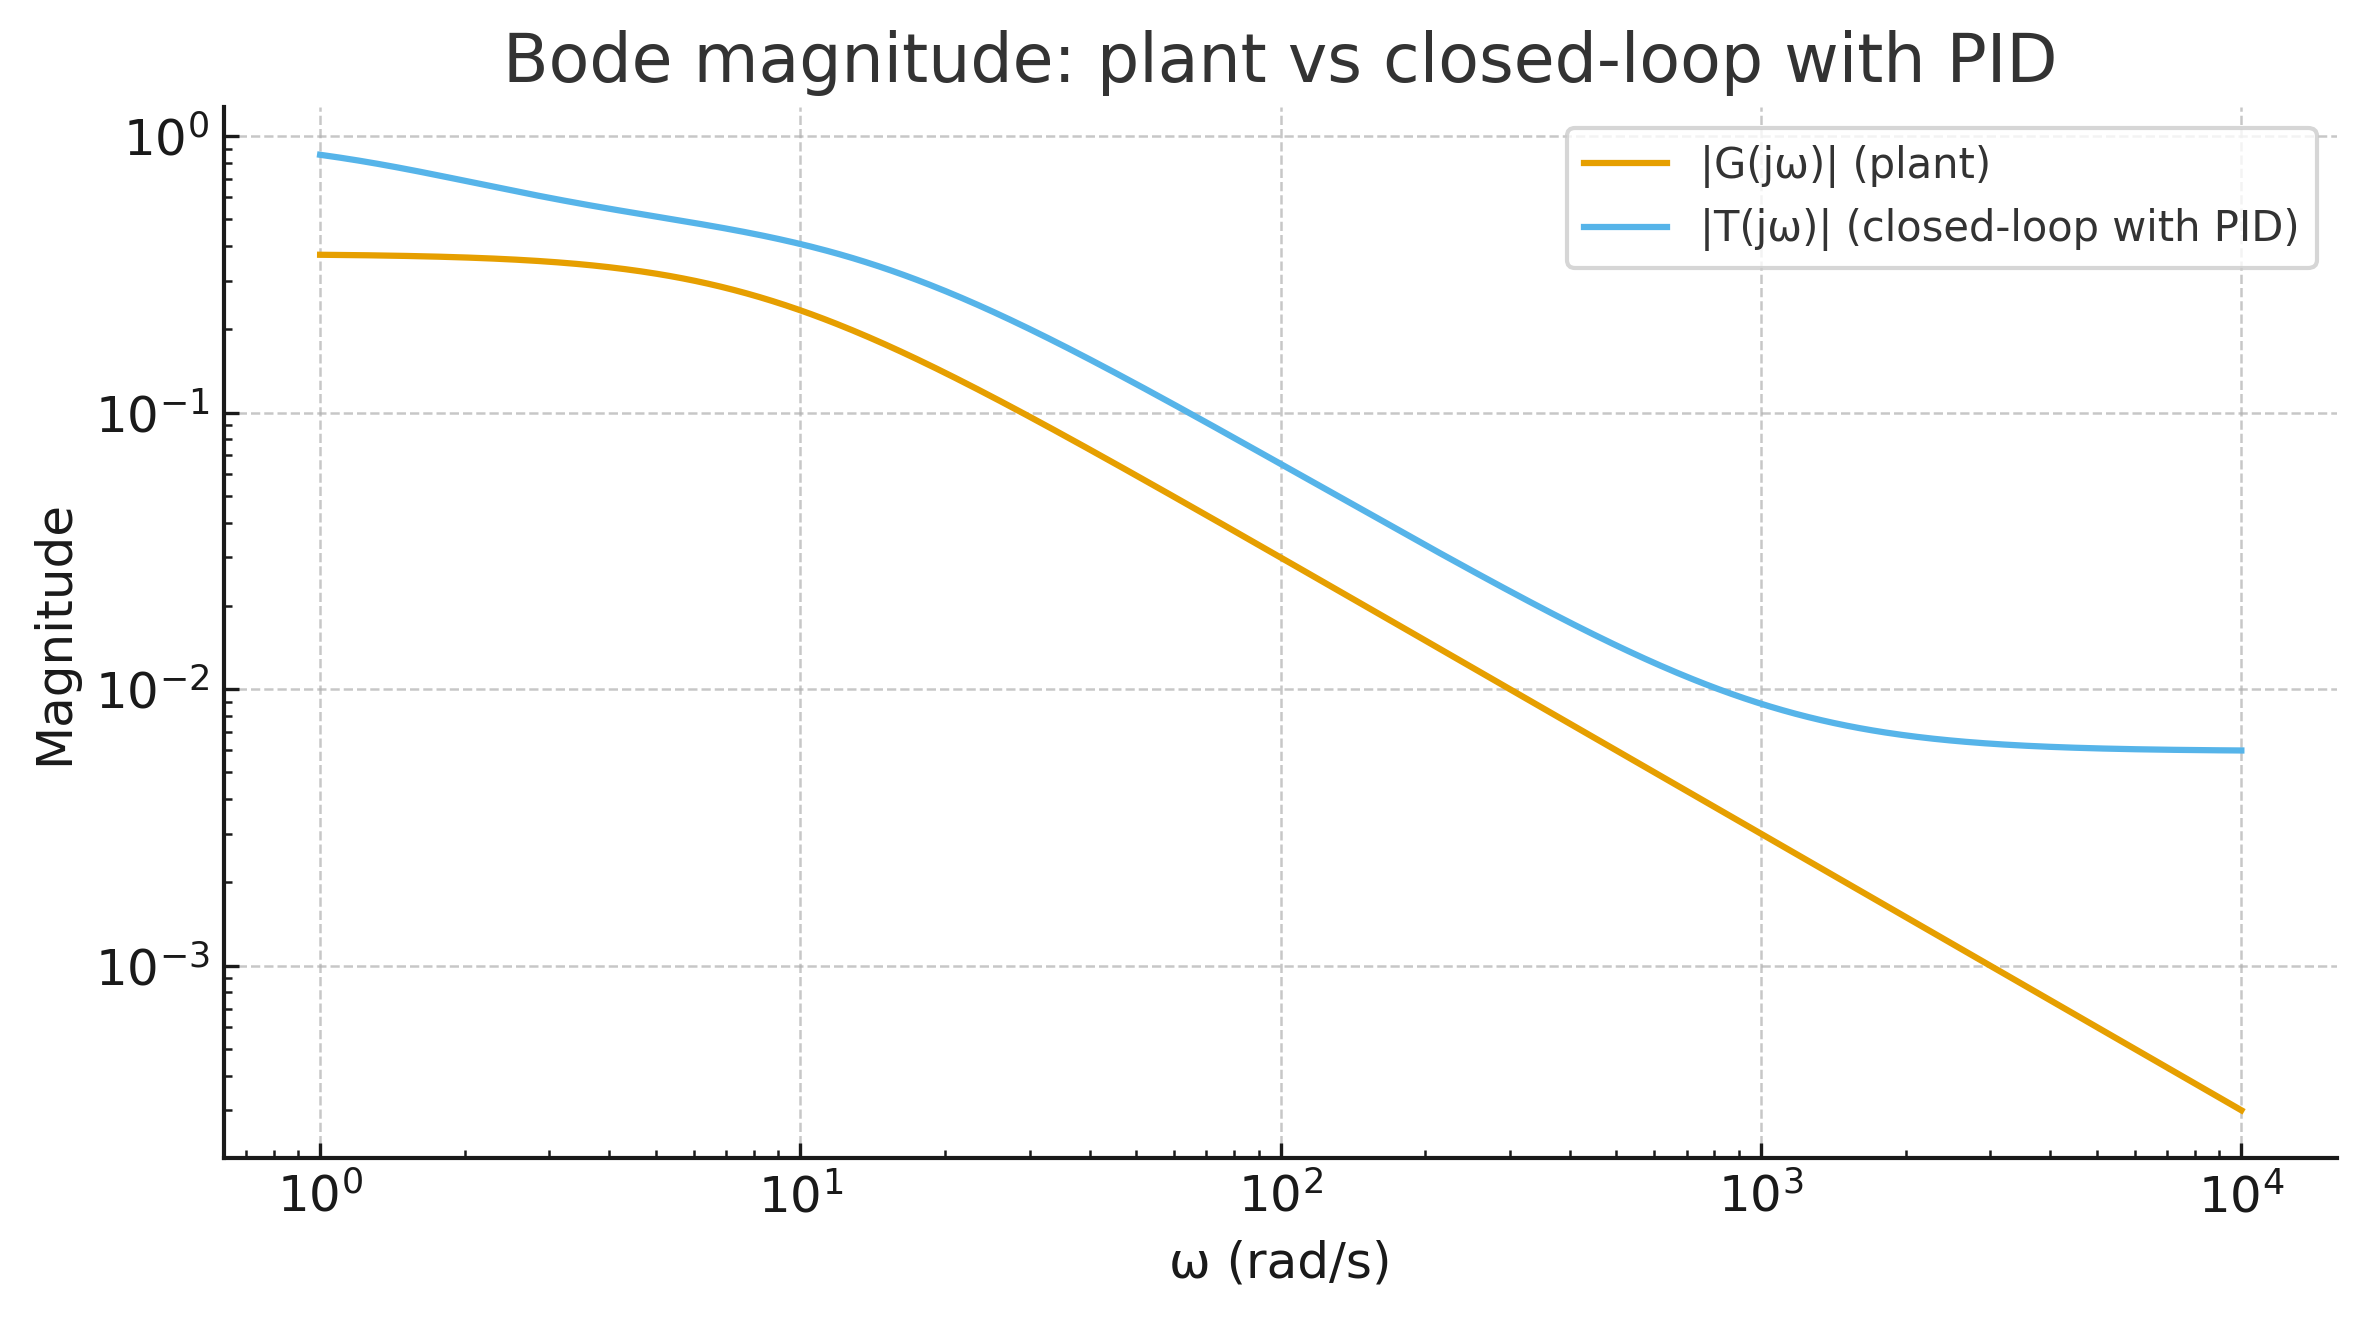
\includegraphics[width=0.9\columnwidth]{fig3_bode_magnitude.png}
\caption{Bode magnitude: plant vs closed-loop with PID.}
\label{fig:bode}
\end{figure}
\begin{table}[h]
\renewcommand{\arraystretch}{1.1}
\caption{Performance Comparison}
\centering
\begin{tabular}{|l|c|c|c|c|}
\hline
Metric & No Ctrl & PID & PID+FSM & PID+FSM+LLM \\
\hline
Peak deviation & $\sim$8\% & $10^{-2}$ & $10^{-3}$ & $2.6\times 10^{-3}$ \\
Steady error   & $10^{-2}$ & $10^{-4}$ & $\sim$0 & $<10^{-6}$ \\
Overshoot      & Large     & Medium    & Small   & Minimal \\
Stress tol.    & None      & Limited   & Medium  & Wide \\
\hline
\end{tabular}
\end{table}

\section{Stability Analysis}
Closed-loop transfer:
\[
T(s) = \frac{L(s)}{1+L(s)}, \quad L(s)=C(s)G(s).
\]
PID ensured phase margin $>45^\circ$, gain margin $>6$ dB. FSM bounded $u$, LLM preserved stability as $\{k_c,\gamma,P\}$ drifted.

\section{Discussion and Limitations}
\subsection{Significance}
Shifts CFET design from static to dynamic compensation.  
\subsection{Comparison with Static Design}
Static methods ignore time evolution; our method uses convergence as design target.  
\subsection{Limitations}
Compact-model abstraction, unmodeled noise/variation, LLM hardware overhead.  
\subsection{Future Work}
Chip-in-loop validation, forksheet/3D CFET extension, integration with cooling and NoC control.  

\section{Conclusion}
We proposed a time-response-aware CFET design with PID+FSM+LLM supervision. Delay and thermal effects were stabilized under dynamic workloads, reframing DTCO from static prediction to dynamic compensation. Time-response-aware design is essential for sub-2\,nm integration.  

\bibliographystyle{IEEEtran}
\bibliography{refs}

\section*{Author Biography}
\noindent\textbf{Shinichi Samizo} received the M.S. degree in Electrical and Electronic Engineering from Shinshu University, Japan. He worked at Seiko Epson Corporation on semiconductor memory and mixed-signal devices, and contributed to inkjet MEMS and PrecisionCore printhead technology. He is now an independent researcher focusing on device physics, memory, and AI-integrated systems.\\
Contact: \href{mailto:shin3t72@gmail.com}{shin3t72@gmail.com}, \href{https://github.com/Samizo-AITL}{Samizo-AITL}
\end{document}
